% ============================================================
\chapter{Recherche de Racines}
\label{ch:racines}
% ============================================================

\section{Exemple motivant}
Trouver $x$ tel que $e^x = 3x$ revient \`a chercher la racine de $f(x)=e^x-3x$. Aucune formule exacte n'existe : il faut une m\'ethode num\'erique.

\section{M\'ethode de bissection}

\begin{theoreme}[Th\'eor\`eme des valeurs interm\'ediaires]\index{bissection}
Si $f\in C([a,b])$ et $f(a)f(b)<0$, alors $\exists\,c\in(a,b)$ tel que $f(c)=0$.
\end{theoreme}

\begin{algorithm}[H]
\caption{Bissection}\label{alg:bissection}
\KwEntree{$f$, $a$, $b$, tol\'erance $\eps$}
\KwSortie{Approximation de la racine $c$}
\While{$b-a > \eps$}{
  $c \gets (a+b)/2$\;
  \eIf{$f(a)\cdot f(c) < 0$}{$b \gets c$}{$a \gets c$}
}
\Return{$c$}
\end{algorithm}

\begin{theoreme}[Convergence de la bissection]
Apr\`es $n$ it\'erations : $|c_n-x^*|\leq\frac{b-a}{2^{n+1}}$. La convergence est \textbf{lin\'eaire} avec taux $1/2$.
\end{theoreme}

\begin{proof}
\`A chaque it\'eration, l'intervalle est divis\'e par 2. Apr\`es $n$ it\'erations, $|I_n|=(b-a)/2^n$ et $|c_n-x^*|\leq|I_n|/2$.
\end{proof}

\section{M\'ethode de Newton}\index{Newton}

\begin{definition}
L'it\'eration de Newton pour $f(x)=0$ est :
\[
x_{n+1} = x_n - \frac{f(x_n)}{f'(x_n)}.
\]
\end{definition}

\begin{center}
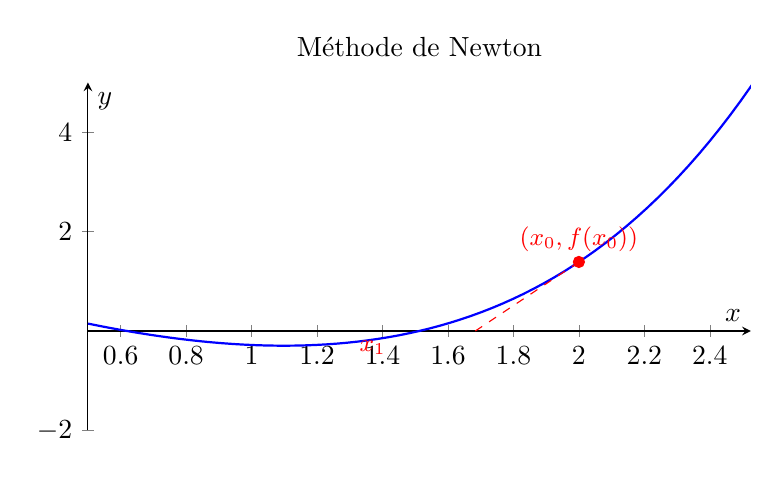
\begin{tikzpicture}
\begin{axis}[
  width=10cm, height=6cm, axis lines=middle,
  xlabel=$x$, ylabel=$y$, ymin=-2, ymax=5,
  domain=0.5:3, samples=80, title={M\'ethode de Newton}
]
\addplot[thick,blue] {exp(x) - 3*x};
\addplot[dashed,red] coordinates {(2,{exp(2)-6}) (2-((exp(2)-6)/(exp(2)-3)),0)};
\addplot[only marks,mark=*,red] coordinates {(2,{exp(2)-6})};
\node[red,below] at (axis cs:1.37,0) {\small $x_1$};
\node[red,above] at (axis cs:2,1.4) {\small $(x_0,f(x_0))$};
\end{axis}
\end{tikzpicture}
\end{center}

\begin{algorithm}[H]
\caption{M\'ethode de Newton}\label{alg:newton}
\KwEntree{$f$, $f'$, $x_0$, tol\'erance $\eps$, $N_{\max}$}
\KwSortie{Approximation $x_n$}
\Pour{$n=0,1,\ldots,N_{\max}$}{
  $x_{n+1} \gets x_n - f(x_n)/f'(x_n)$\;
  \Si{$|x_{n+1}-x_n|<\eps$}{\Return{$x_{n+1}$}}
}
\end{algorithm}

\begin{theoreme}[Convergence quadratique de Newton]\label{thm:newton-conv}
Si $f\in C^2$, $f(x^*)=0$, $f'(x^*)\neq 0$ et $x_0$ suffisamment proche de $x^*$, alors :
\[
|e_{n+1}| \leq \frac{M}{2m}|e_n|^2,
\]
o\`u $e_n=x_n-x^*$, $M=\sup|f''|$, $m=\inf|f'|$ au voisinage de $x^*$.
\end{theoreme}

\begin{proof}
Par Taylor : $0=f(x^*)=f(x_n)+f'(x_n)(x^*-x_n)+\frac{f''(\xi_n)}{2}(x^*-x_n)^2$. Divisant par $f'(x_n)$ :
\[
0 = \frac{f(x_n)}{f'(x_n)}+(x^*-x_n)+\frac{f''(\xi_n)}{2f'(x_n)}e_n^2.
\]
Or $x_{n+1}=x_n-f(x_n)/f'(x_n)$, donc $e_{n+1}=x_{n+1}-x^*=-\frac{f''(\xi_n)}{2f'(x_n)}e_n^2$.
\end{proof}

\section{M\'ethode de la s\'ecante}\index{secante@s\'ecante}

\begin{definition}
On remplace $f'(x_n)$ par une diff\'erence finie :
\[
x_{n+1} = x_n - f(x_n)\frac{x_n-x_{n-1}}{f(x_n)-f(x_{n-1})}.
\]
\end{definition}

\begin{theoreme}
L'ordre de convergence de la s\'ecante est le \textbf{nombre d'or} $\varphi=(1+\sqrt{5})/2\approx 1{,}618$.
\end{theoreme}

\section{M\'ethode du point fixe}\index{point fixe}

\begin{definition}
Trouver $x=g(x)$. It\'eration : $x_{n+1}=g(x_n)$.
\end{definition}

\begin{theoreme}[Th\'eor\`eme du point fixe de Banach]\label{thm:banach}
Si $g:[a,b]\to[a,b]$ est une contraction ($|g'(x)|\leq L<1$ sur $[a,b]$), alors $g$ a un unique point fixe $x^*$ et $x_n\to x^*$ avec :
\[
|x_n-x^*|\leq \frac{L^n}{1-L}|x_1-x_0|.
\]
\end{theoreme}

\section{Comparaison des m\'ethodes}

\begin{center}
\begin{tabular}{lccc}
\toprule
\textbf{M\'ethode} & \textbf{Ordre} & \textbf{Appels $f$} & \textbf{Robustesse} \\
\midrule
Bissection & 1 (lin\'eaire) & 1/it. & Tr\`es robuste \\
Newton & 2 (quadratique) & $f + f'$/it. & Sensible \`a $x_0$ \\
S\'ecante & $\varphi\approx 1{,}618$ & 1/it. & Mod\'er\'ee \\
\bottomrule
\end{tabular}
\end{center}

\section{Exemple num\'erique}

Racine de $f(x)=e^x-3x$ avec $x_0=2$ (Newton) :
\begin{center}
\begin{tabular}{cccc}
\toprule
$n$ & $x_n$ & $f(x_n)$ & $|x_n-x_{n-1}|$ \\
\midrule
0 & 2.000000 & 1.389056 & --- \\
1 & 1.373418 & 0.225698 & 0.627 \\
2 & 1.524247 & $-0.046$ & 0.151 \\
3 & 1.512127 & $-0.000374$ & 0.012 \\
4 & 1.512135 & $<10^{-9}$ & $8\times10^{-6}$ \\
\bottomrule
\end{tabular}
\end{center}

\section{Impl\'ementation}

\begin{codeblock}[title=\textbf{Python}]
\begin{minted}{python}
import numpy as np

def bisection(f, a, b, tol=1e-12):
    while b - a > tol:
        c = (a + b) / 2
        if f(a) * f(c) < 0:
            b = c
        else:
            a = c
    return (a + b) / 2

def newton(f, df, x0, tol=1e-12, maxiter=100):
    x = x0
    for i in range(maxiter):
        dx = f(x) / df(x)
        x -= dx
        if abs(dx) < tol:
            return x, i+1
    return x, maxiter

def secant(f, x0, x1, tol=1e-12, maxiter=100):
    for i in range(maxiter):
        fx0, fx1 = f(x0), f(x1)
        x2 = x1 - fx1 * (x1 - x0) / (fx1 - fx0)
        if abs(x2 - x1) < tol:
            return x2, i+1
        x0, x1 = x1, x2
    return x1, maxiter

# Test
f = lambda x: np.exp(x) - 3*x
df = lambda x: np.exp(x) - 3

print(f"Bissection : {bisection(f, 0, 1):.12f}")
x_newton, n = newton(f, df, 2.0)
print(f"Newton     : {x_newton:.12f} ({n} iterations)")
x_sec, n = secant(f, 0.0, 1.0)
print(f"Secante    : {x_sec:.12f} ({n} iterations)")
\end{minted}
\end{codeblock}

\begin{codeblock}[title=\textbf{Julia}]
\begin{minted}{julia}
function newton(f, df, x0; tol=1e-12, maxiter=100)
    x = x0
    for i in 1:maxiter
        dx = f(x) / df(x)
        x -= dx
        abs(dx) < tol && return x, i
    end
    return x, maxiter
end

f(x) = exp(x) - 3x
df(x) = exp(x) - 3
x, n = newton(f, df, 2.0)
println("Newton: x = $x ($n iterations)")
\end{minted}
\end{codeblock}

\section{Exercices}

\begin{exercice}[$\star$]
Trouver $\sqrt{2}$ par Newton appliqu\'e \`a $f(x)=x^2-2$. Combien d'it\'erations pour 15 d\'ecimales ?
\end{exercice}

\begin{exercice}[$\star\star$]
Montrer que Newton appliqu\'e \`a $f(x)=x^2$ converge lin\'eairement (racine double). G\'en\'eraliser : que se passe-t-il quand $f'(x^*)=0$ ?
\end{exercice}

\begin{exercice}[$\star\star$]
D\'emontrer l'ordre $\varphi$ de la s\'ecante en posant $e_{n+1}\approx C\,e_n^p$ et en r\'esolvant $p^2-p-1=0$.
\end{exercice}

\begin{exercice}[$\star\star\star$ -- Projet]
Impl\'ementer la m\'ethode de Brent (combinaison bissection + s\'ecante). Comparer avec les m\'ethodes simples sur 10 fonctions test.
\end{exercice}

\begin{formules}
\begin{align*}
\text{Bissection} &: |e_n|\leq\frac{b-a}{2^{n+1}} \\
\text{Newton} &: x_{n+1}=x_n-\frac{f(x_n)}{f'(x_n)},\quad |e_{n+1}|\leq C|e_n|^2 \\
\text{S\'ecante} &: x_{n+1}=x_n-f(x_n)\frac{x_n-x_{n-1}}{f(x_n)-f(x_{n-1})},\quad \text{ordre }\varphi
\end{align*}
\end{formules}
